We consider a continuous spatial variable in $\mathbb{R}^1$ s.t. 
\begin{align*}
    \{r(x): x \in \text{D} &: [1,50] \subset \mathbb{R}^1\} \\
    \E\{r(x)\} &= \mu_r = 0\\
    \Var\{r(x)\} & = \sigma_r^2 \\
    \Corr\{r(x), r(x')\} & = \rho_r(\tau) \, ,
\end{align*}

where $\tau = |x-x^\prime|/10.$ 
Discretization: $\text{L} \in \{1,2,...,50\}$.
The discretized random field (RF) is 
\begin{equation*}
    \{r(x): x \in \text{L}\}.
\end{equation*}

\paragraph{a)}
A function $c(\vect{\tau}) : \R^q \rightarrow \R$ is positive definite (non-negative definite, to be precise) for $\vect{\tau} \in \R^q$ if
%
\begin{equation*}
\begin{split}
    & \sum_{i=1}^n \sum_{j=1}^n \alpha_i \alpha_j c(\vect{x_i} - \vect{x_j}) \geq 0 \\
    & \forall [\vect{x}_1, \vect{x}_2, \dots, \vect{x}_n] \in \R^{q \times n} \\
    & \forall \vect{\alpha} \in \R^n \\
    & \forall n \in \mathbb{N}_+ \setminus \{1\} \, .
\end{split}
\end{equation*}
%
In one dimension we replace the vectors $\vect{\tau}, \vect{x}_i$ and $\vect{x}_j$ with scalars $\tau, x_i$ and $x_j$.

Now assume that $\sum_{i=1}^n \sum_{j=1}^n \alpha_i \alpha_j \rho_r(\tau) < 0$ for some $[x_1, x_2, \dots, x_n]$, $\vect{\alpha}$ and $n$. Then
%
\begin{align*}
    \Var\left(\sum_{i=1}^n \alpha_i r(x_i)\right) 
    &= \sum_{i=1}^n \sum_{j=1}^n \alpha_i \alpha_j \Cov\{r(x_i), r(x_j)\} \\
    &= \sum_{i=1}^n \sum_{j=1}^n \alpha_i \alpha_j \sigma^2_r \Corr\{r(x_i), r(x_j)\} \\
    &= \sigma^2_r \sum_{i=1}^n \sum_{j=1}^n \alpha_i \alpha_j \rho_r(\tau) \\
    &< 0 \, .
\end{align*}
%
But the variance of a weighted sum of random variables is non-negative, so this is a contradiction. Thus the correlation function needs to be positive definite.

Two possible correlation functions, $\rho_r(\tau)$, the Powered exponential and the Matern. The functions take values for $\tau$, and a parameter $\nu_r$. Let $\nu_r \in \{1,3\}$ for the Matern function and $\nu_r \in \{1,1.9\}$ for Powered exponential. 

The correlation functions for each $\nu_r$ are shown in figure \ref{fig:corrfunc}. We see that the correlation is 1 for $\tau = 0$ and goes to 0 as $\tau$ increases for all the function and parameter configurations, as desired.

Cruical features for the spatial correlation function...?

\begin{figure}
    \centering
    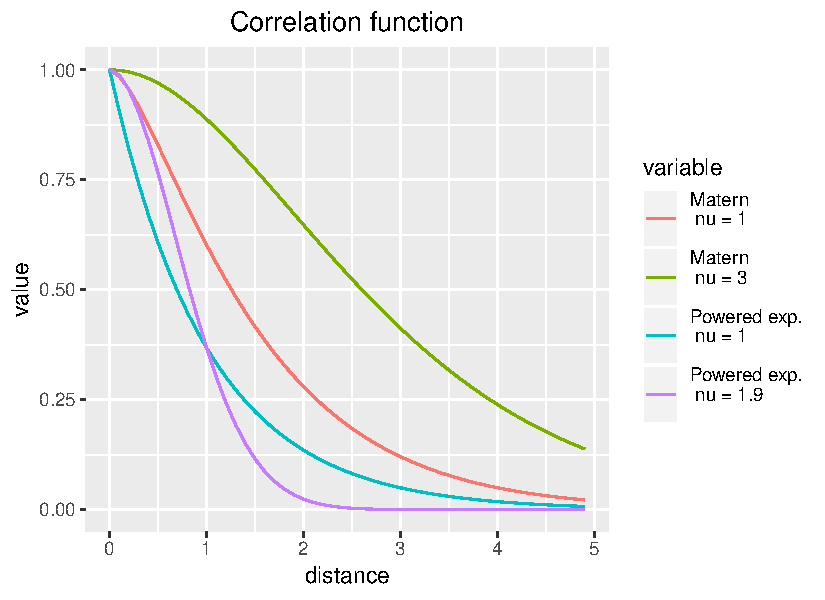
\includegraphics{figures/corrfunc.pdf}
    \caption{The Powered exponential and the Matern spatial correlation functions for some parameter values.}
    \label{fig:corrfunc}
\end{figure}

The variogram function is
%
\begin{align*}
\gamma_r(\tau)
\coloneqq&\: \frac{1}{2} \Var \{ r(x) - r(x') \} \\
=&\: \sigma_r^2 - \Cov\{r(x), r(x')\} \\
=&\: \sigma_r^2[1 - \rho_r(\tau)]\, ,
\end{align*}
%
i.e. 1 minus the correlation scaled by the variance.
This is displayed for the given parameter values in figure \ref{fig:variograms}.

\begin{figure}
    \centering
    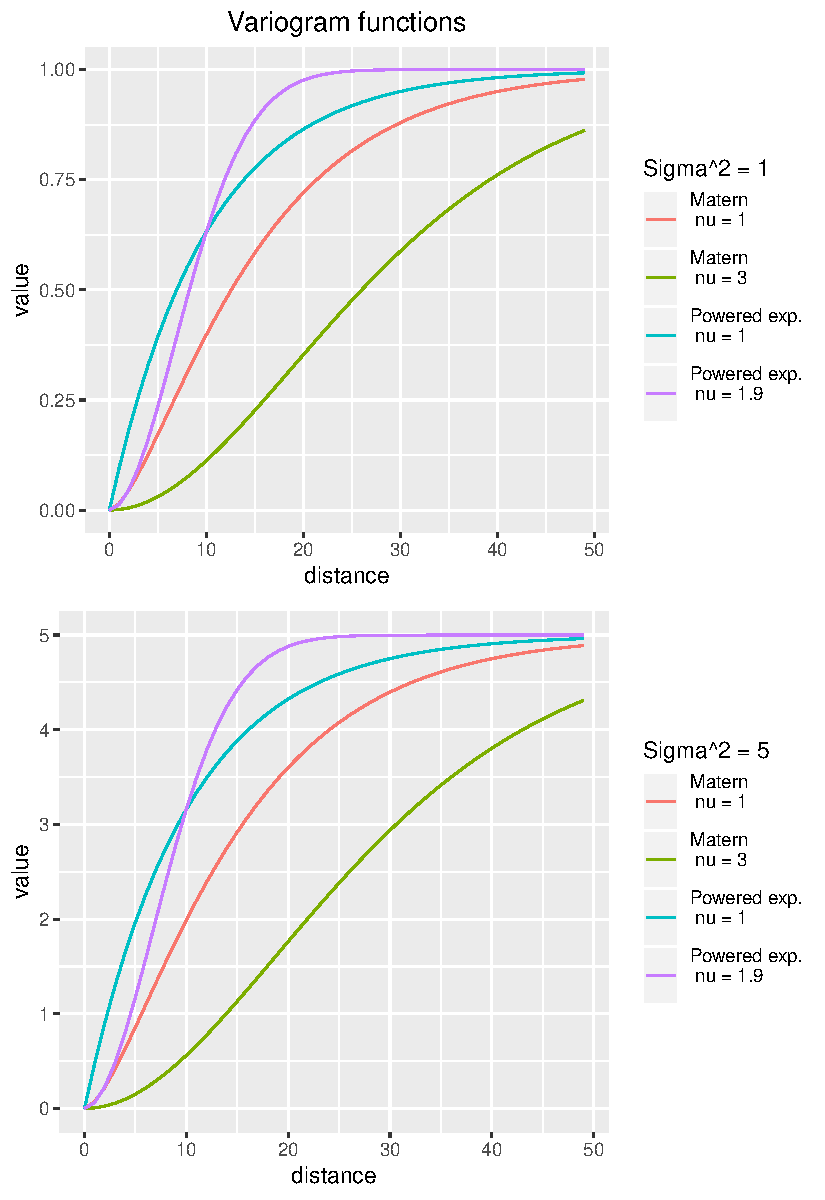
\includegraphics{figures/variograms.pdf}
    \caption{The variogram functions corresponding to Powered exponential and the Matern spatial correlation functions for some parameter values. The variance, $\\sigma^2$, is purely scaling the functions.}
    \label{fig:variograms}
\end{figure}





%%%%%%%%%%%%%%%%%%%%%%%%%%%%%%%%%%%%%%%%%%%%%%%%%%%%%%%%%%%%%%%%%%%%%%
\paragraph{b)}
The discretized prior Gaussian model has pdf
\begin{equation}
    \vect{r} \sim p(\vect{r}) = \phi_n(\vect{r}; \mu_r \vect{i}_n, \sigma_r^2\matr{\Sigma}_r^{\rho}),
\end{equation}
where $n = 50$ is the number of grid points in $\text{L},$ $\vect{i}_n$ is a $n$-vector with $1$s and $\matr{\Sigma}_r^{\rho}$ is the correlation matrix for the grid points, defined from the chosen spatial correlation function applied to all $\tau$s in the system.

Ten realizations for each of the eight different parameter combinations are displayed in figures \ref{fig:prior_samp_exp} and \ref{fig:prior_samp_matern}. The priors in figure \ref{fig:prior_samp_exp} are using the Powered exponential function as correlation function, while the ones in figure \ref{fig:prior_samp_matern} use the Matern correlation function.

The influence of the parameter values are illustrated in the plots. Large $\sigma^2$ means large variability in values, and the realizations vary more along the $y$-axis in these displays. Increased $\nu_r$ increases the correlation between space points, as shown in figure \ref{fig:corrfunc}. Thus, this results in smoother realizations, where changes are done more gradually.

\begin{figure}[]
\centering
    \begin{subfigure}[H]{0.49\textwidth}
        \centering
        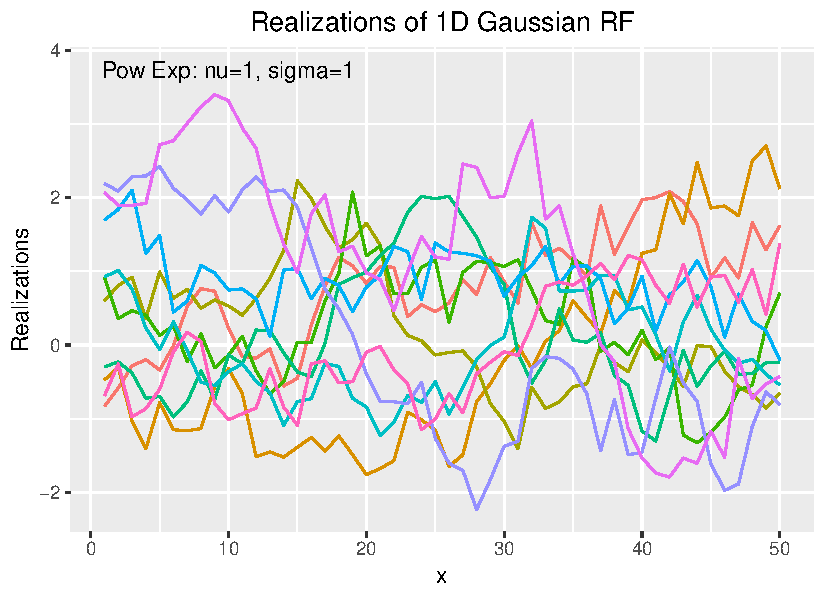
\includegraphics[scale=0.5,trim=0cm 0cm 0cm 0cm]{figures/sample1conf1.pdf}
    \end{subfigure}
    \hfill
    \begin{subfigure}[H]{0.49\textwidth}  
        \centering 
        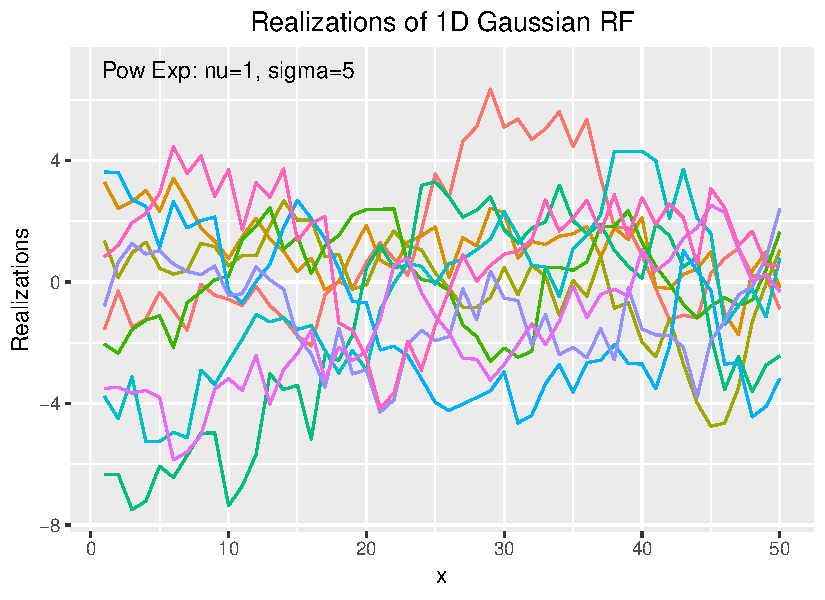
\includegraphics[scale=0.5,trim=0cm 0cm 0cm 0cm]{figures/sample1conf2.pdf}
    \end{subfigure}

    \vskip\baselineskip
    
     \begin{subfigure}[H]{0.49\textwidth}
        \centering
        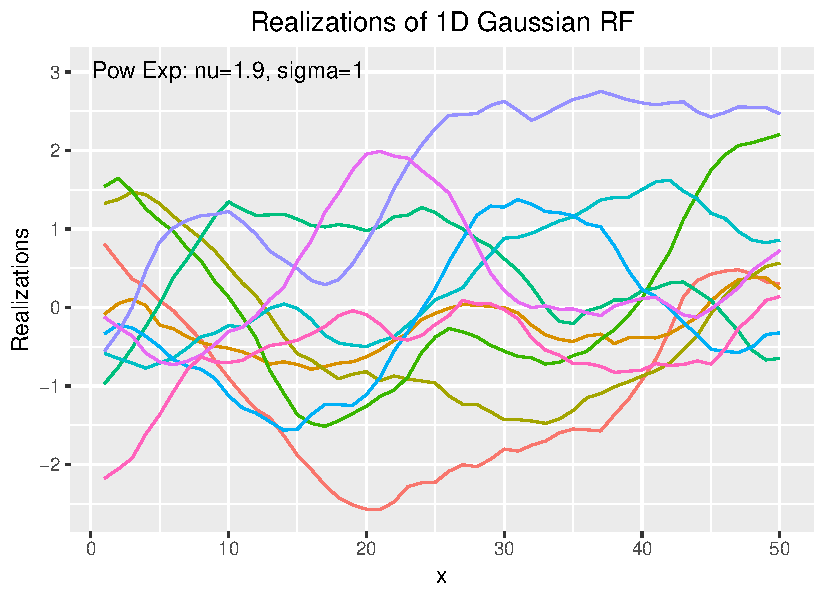
\includegraphics[scale=0.5,trim=0cm 0cm 0cm 0cm]{figures/sample1conf3.pdf}
    \end{subfigure}
    \hfill
    \begin{subfigure}[H]{0.49\textwidth}  
        \centering 
        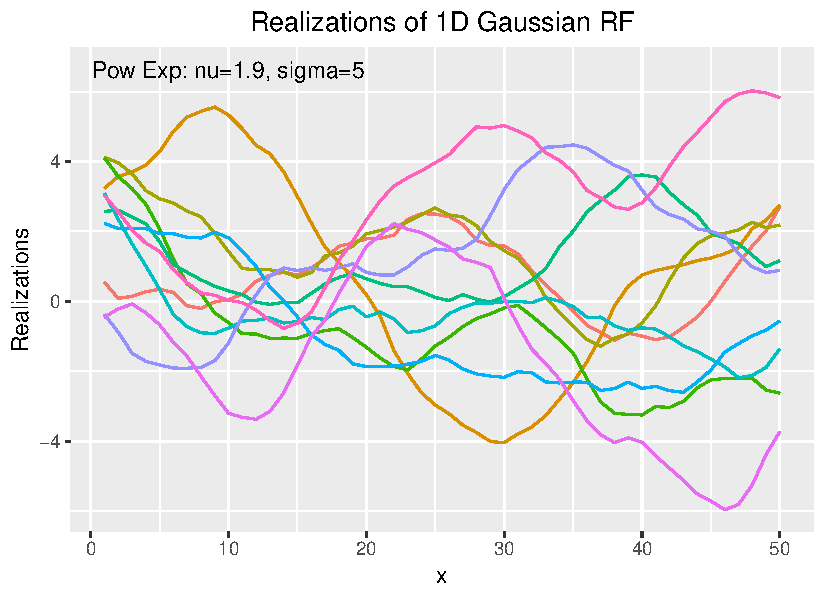
\includegraphics[scale=0.5,trim=0cm 0cm 0cm 0cm]{figures/sample1conf4.pdf}
    \end{subfigure}

    \caption{Realizations from prior Gaussian RF using Powered exponential correlation function. Model parametere values are shown the each plot, respectively.}
    \label{fig:prior_samp_exp}
\end{figure}

\begin{figure}[]
\centering
    \begin{subfigure}[H]{0.49\textwidth}
        \centering
        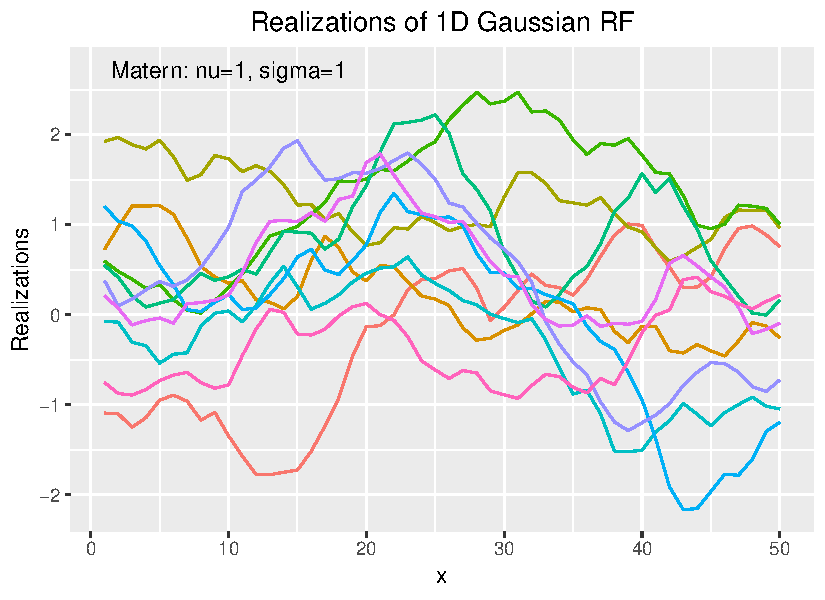
\includegraphics[scale=0.5,trim=0cm 0cm 0cm 0cm]{figures/sample1conf5.pdf}
    \end{subfigure}
    \hfill
    \begin{subfigure}[H]{0.49\textwidth}  
        \centering 
        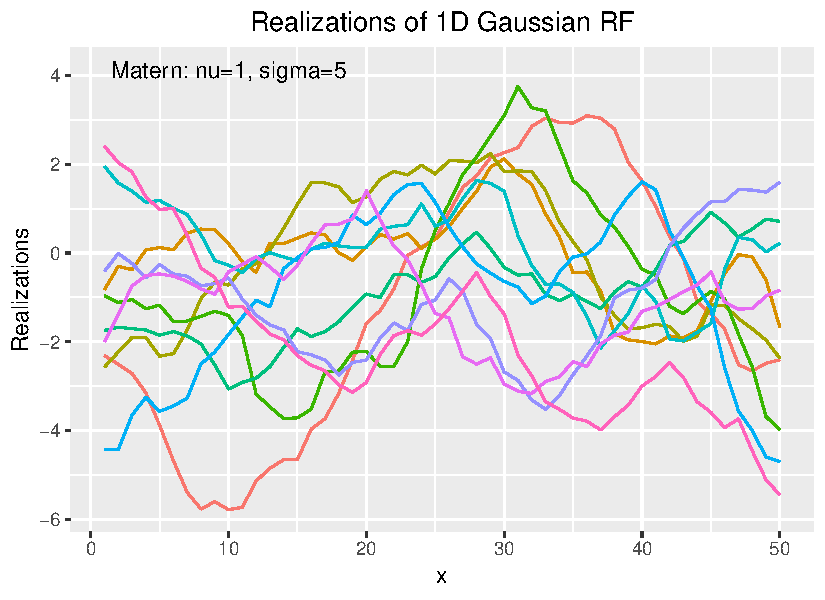
\includegraphics[scale=0.5,trim=0cm 0cm 0cm 0cm]{figures/sample1conf6.pdf}
    \end{subfigure}

    \vskip\baselineskip
    
     \begin{subfigure}[H]{0.49\textwidth}
        \centering
        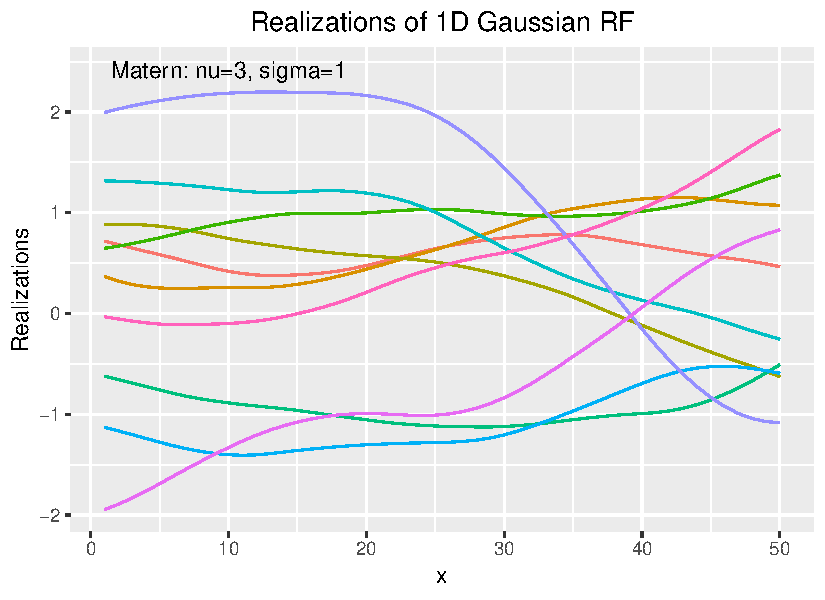
\includegraphics[scale=0.5,trim=0cm 0cm 0cm 0cm]{figures/sample1conf7.pdf}
    \end{subfigure}
    \hfill
    \begin{subfigure}[H]{0.49\textwidth}  
        \centering 
        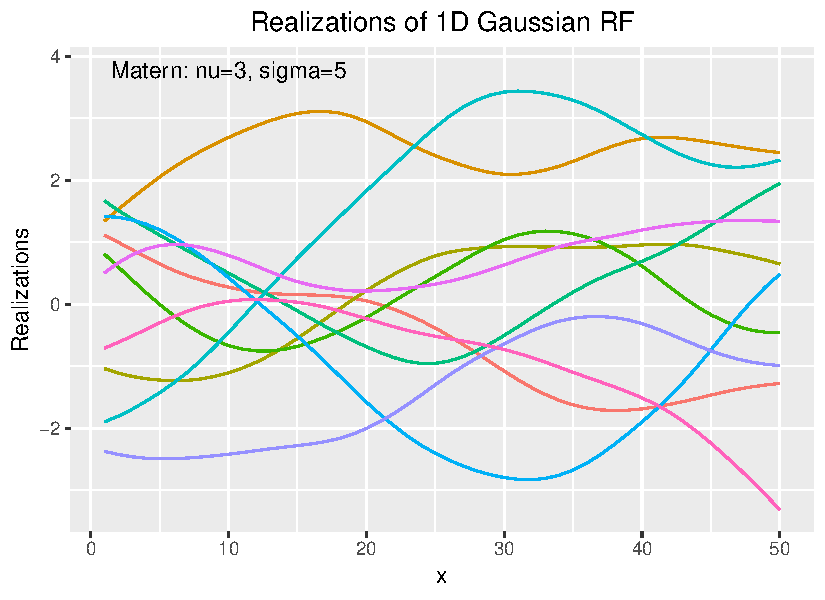
\includegraphics[scale=0.5,trim=0cm 0cm 0cm 0cm]{figures/sample1conf8.pdf}
    \end{subfigure}

    \caption{Realizations from prior Gaussian RF using Matern correlation function. Model parametere values are shown the each plot, respectively.}
    \label{fig:prior_samp_matern}
\end{figure}

%%%%%%%%%%%%%%%%%%%%%%%%%%%%%%%%%%%%%%%%%%%%%%%%%%%%%%%%%%%%%%%%%%%%%%
\paragraph{c)}
Now assume the spatial variable is observed as 
\begin{align*}
    \{&d(x): x \in \{10,25,30\} \subset \text{L} \}\\
    &d(x) = r(x) + \epsilon(x),
\end{align*}
where the measurement errors, $\epsilon(\cdot)$, are independent and identically distributed.
\begin{equation*}
    \epsilon(x) \sim \phi(\epsilon; 0,\sigma^2_{\epsilon}).
\end{equation*}
$r(x)$ and $\epsilon(x^\prime)$ are also independent for all $x,x^\prime$.

The likelihood function for this model is the Gauss-linear likelihood.
\begin{equation}
    [\vect{d}|\vect{r}] = \matr{H}\vect{r} + \vect{\epsilon} \sim p(\vect{d}|\vect{r}) = 
    \phi_m\left(\vect{d};\matr{H}\vect{r}, \matr{\Sigma}_{d|r}\right).
\end{equation}
$m$ is the dimension of $\vect{d}|\vect{r}$, $\matr{H}$ is the observation matrix with dimensions $m \times n$, and $\matr{\Sigma}_{d|r} = \sigma^2_{\epsilon} \matr{I}_m$, $\matr{I}_m$ being the $m \times m$ identity matrix.

The likelihood $p(\vect{d}|\vect{r})$ would be a pdf as a function of the data, but in this setting, the data is known and constant and $\vect{r}$ is unknown. Thus, the likelihood should be considered a function of $\vect{r}$. As a function of $\vect{r}$, it does noe necessarily integrate to $1$, and hence it is not a pdf. Because of this, there is no need to normalize the likelihood function.


%%%%%%%%%%%%%%%%%%%%%%%%%%%%%%%%%%%%%%%%%%%%%%%%%%%%%%%%%%%%%%%%%%%%%%
\paragraph{d)}
To simulate that $\{d(x): x \in \{10,25,30\} \subset \text{L} \}$  is observed, one realization from problem 1b) is saved. The realization is chosen from the prior with parameter combination $\sigma^2 = 5$ and Powered exponential correlation function with $\nu_r = 1.9$. We also let $\sigma^2_{\epsilon} \in \{0,0.25\}$.

The Gaussian RF is a conjugate prior class to the Gauss-linear likelihood. Thus, the posterior distribution is also a Gaussian RF. The Gaussian distribution is completely determined by the mean and the variance. For the discretized version we have
\begin{align*}
    [\vect{r}|\vect{d}] &\sim p(\vect{r}|\vect{d}) = \phi_n\left(\vect{r};\vect{\mu}_{r|d}, \matr{\Sigma}_{r|d}\right), \text{ with }\\
    \vect{\mu}_{r|d} &= \mu_r\vect{i}_n + \sigma^2_r\matr\Sigma^{\rho}_r\matr{H}^T \left[\sigma^2_r\matr{H}\matr\Sigma^{\rho}_r\matr{H}^T + \matr{\Sigma}_{d|r}\right]^{-1}[\vect{d}-\mu_r\matr{H}\vect{i}_n]\\
    \matr{\Sigma}_{r|d} &= \sigma^2_r\matr\Sigma^{\rho}_r - \sigma^2_r\matr\Sigma^{\rho}_r\matr{H}^T \left[\sigma^2_r\matr{H}\matr\Sigma^{\rho}_r\matr{H}^T + \matr{\Sigma}_{d|r}\right]^{-1} \sigma^2_r\matr{H} \matr\Sigma^{\rho}_r
\end{align*}

For prediction, the posterior mean is commonly used. The associated $(1-\alpha)$ prediction interval is 
$$\left[\vect{\mu_{r|d}}-z_{\alpha/2} \sqrt{diag(\matr{\Sigma_{r|d}})},\quad \vect{\mu_{r|d}}+z_{\alpha/2} \sqrt{diag(\matr{\Sigma_{r|d}})}\right].$$

Predicted values with corresponding prediction intervals for the two measurement errors are shown in figure \ref{fig:predictions}.

\begin{figure}
    \centering
    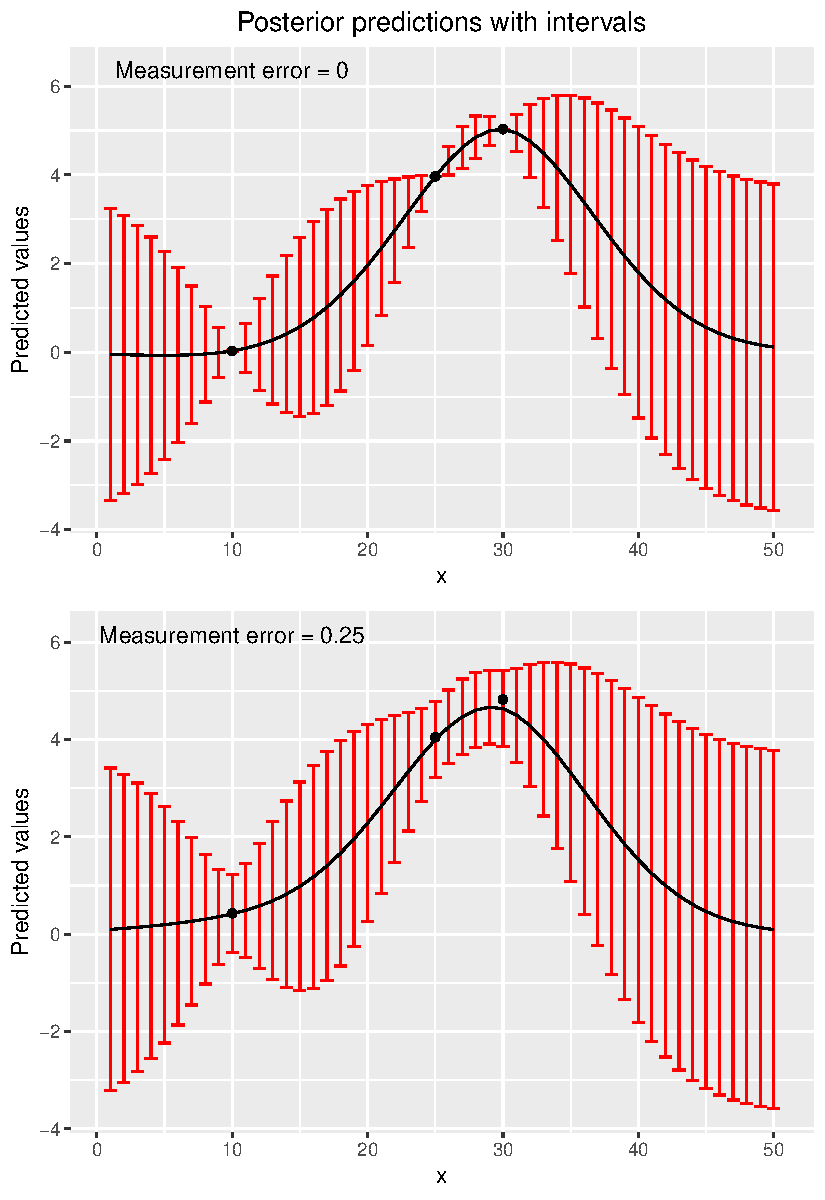
\includegraphics{figures/predictions.pdf}
    \caption{Posterior mean and prediction intervals for two different measurment errors when measured in $x = \{10,25,30\}$. The measured values are shown in black dots.}
    \label{fig:predictions}
\end{figure}

The measurement error has an effect in the posterior predictions in several ways. The measurement errors means that different values can be drawn from the same system in the same positions, and the error affects both the mean and the variance in the posterior distribution. In particular, notice that when the measurement error $\sigma^2_{\epsilon} = 0$, the posterior mean in the measured positions matches the measured values in this places, and there is no uncertainty in these positions. The uncertainty increases with the distance from the measured positions.

%%%%%%%%%%%%%%%%%%%%%%%%%%%%%%%%%%%%%%%%%%%%%%%%%%%%%%%%%%%%%%%%%%%%%%
\paragraph{e)}

The predictions from problem 1d) can be estimated by simulate realizations from the posterior distribution and computing the empirical mean and standard deviation from the realizations. 
The result is shown in figure \ref{fig:postSamps}.

\begin{figure}
    \centering
    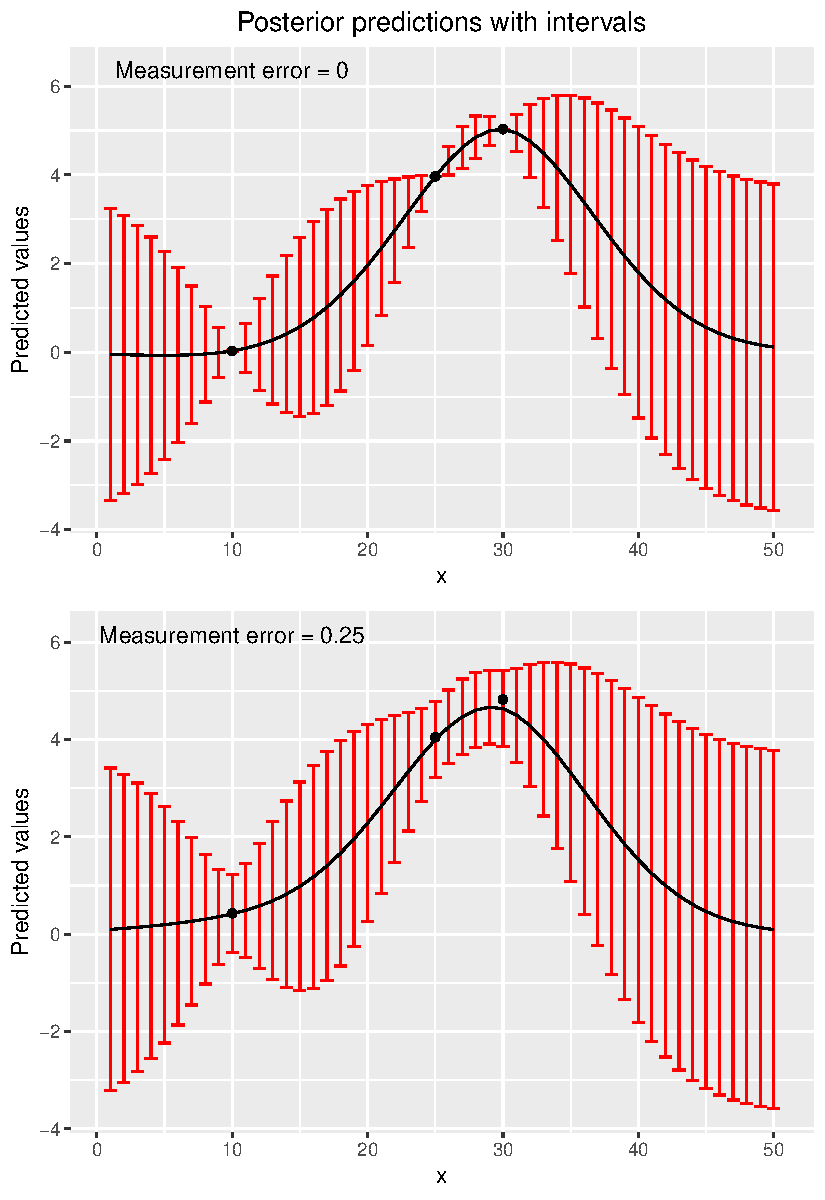
\includegraphics{figures/predictions.pdf}
    \caption{Posterior mean and prediction intervals for two different measurment errors when measured in $x = \{10,25,30\}$. The measured values are shown in black dots.}
    \label{fig:postSamps}
\end{figure}


%%%%%%%%%%%%%%%%%%%%%%%%%%%%%%%%%%%%%%%%%%%%%%%%%%%%%%%%%%%%%%%%%%%%%%
\paragraph{f)}
text text text

%%%%%%%%%%%%%%%%%%%%%%%%%%%%%%%%%%%%%%%%%%%%%%%%%%%%%%%%%%%%%%%%%%%%%%
\paragraph{g)}
text text text
